\section{Theorie}
\subsection{Grundlagen}
Brechung finden statt, wenn eine elektromagnetische Welle mit einem elektrischen Feldvektor $\vec{E}(\vec{r})=\vec{E}_0e^{i\vec{k}\vec{r}}$ von einem Medium in ein anderes ($n_2=n\neq1$) wechselt. Für den Bereich der Röntgenstrahlung liegt die Wellenlänge zwischen $\lambda=\SI{0,1}{\AA}$ und $\lambda=\SI{10}{\AA}$; der Brechungsindex kann als
\begin{equation*}
  n=1-\delta+i\beta
  \label{eq:brechungsindex}
\end{equation*}
geschrieben werden. Der Korrekturterm $\delta$ liegt in der Größenordnung $10^{-6}$. $\beta$ beschreibt die Absorption und liegt bei der für diesen Versuch genutzte Strahlungsenergie von $E=\SI{8}{keV}$ in einer Größenordnung von $10^{-7}$. Somit ist der Realteil des Brechungsindexes für Röntgenstrahlung immer kleiner als 1. Dies ermöglicht das Ausnutzen der auftretenden äußeren Totalreflexion. Aus dem Snelliusschen Brechungsgesetz
\begin{equation*}
\frac{n_1}{n_2}=\frac{\cos(\alpha_t)}{\cos(\alpha_i)}\quad\text{mit}\; (n_1=n_\text{Vak}=1)
\label{eq:snellius}
\end{equation*}
 und einer idealisierten Annahme, dass es sich um homogene Schichten handelt, ergibt sich ein kritischer Winkel, unter dem die Totalreflexion auftritt. Wird von kleinen Winkeln ausgegangen, so tritt diese bei $a_C\approx\sqrt{2\delta}=\lambda\sqrt{\frac{r_e\rho}{\pii}}$
 auf. $\lambda$ ist die Wellenlänge der Strahlung, $\rho$ die Elektronendichte des Materials und $r_e$ der Elektronenradius.
 \begin{figure}[H]
   \centering
   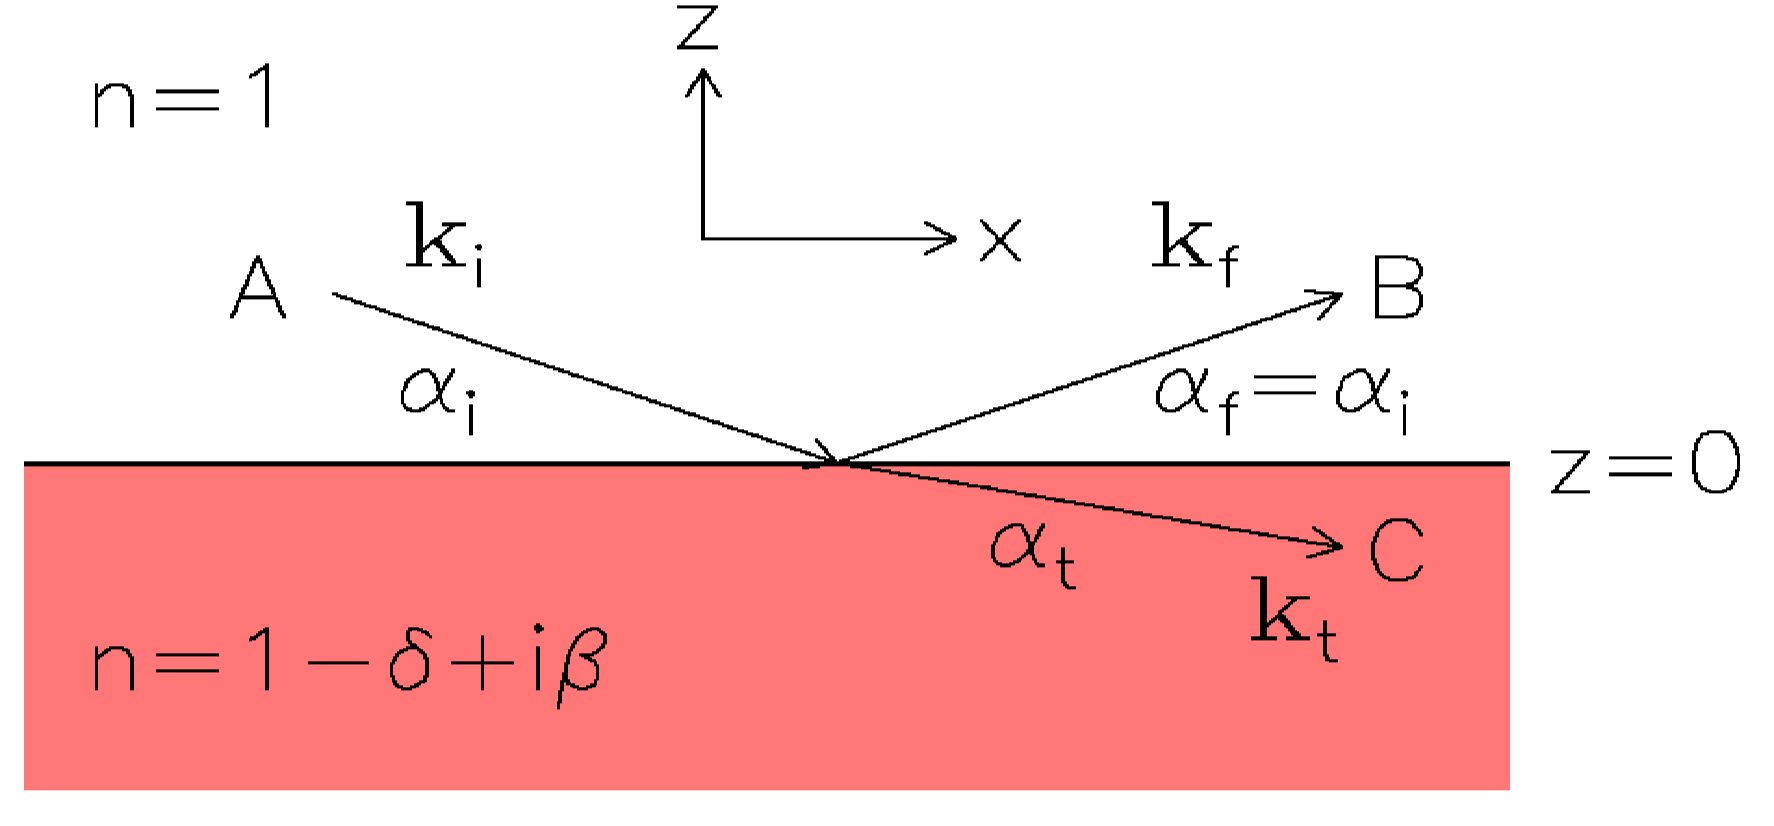
\includegraphics[width=0.7\textwidth]{bilder/schema1.png}
   \caption{Schematische Darstellung für die Reflexion und Transmission einer elektromagnetischen Welle unter Einzeichnung aller bereits benannten Größen, die diesen Zusammenhang für die Brechung beschreiben\cite{anleitung}.}
   \label{schema1}
 \end{figure}
Wird im Allgemeinen eine solche Reflektivität beschrieben, so muss stets die Polarisation des einfallenden Lichts berücksichtigt werden. Den physikalischen Zusammenhang beschreiben die Fresnel-Formeln. Unter der Annahme, dass mit s-polarisierter Strahlung gearbeitet wird, ergibt sich
\begin{align}
  r_S&=\frac{B}{A}=\frac{k_{i,z}-k_{t,z}}{k_{i,z}+k_{t,z}}\\
  t_S&=\frac{C}{A}=\frac{2k_{i,z}}{k_{i,z}+k_t,z}.
\end{align}
Hierbei sind $k_{i,z}=k\sin(\alpha_i)$ und $k_{t,z}=nk\sin(\alpha_t)=k\sqrt{n^2-\cos^2(\alpha_i)}$ mit der Wellenzahl $k=\frac{2\pii}{\lambda}$. Eine Unterscheidung bei Röntgenstrahlung zwischen den Polarisationsrichtungen s und p sind nicht nötig, da der Unterschied in den Fresnel-Gleichungen aufgrund von $n_2\approx n_1$ vernachlässigbar klein ist.
Da die Intensität $I$ proportional zum Betragsquadrat der Feldstärke ist, wird das Verhältnis zwischen der Intensität der reflektierten $I_R$ und der einfallenden Strahlung $I_0$ durch
\begin{equation}
  R=\frac{I_R}{I_0}=|r|^2
\end{equation}
angegeben. Die Fresnelreflektivität ist für Röntgenstrahlung und für $\alpha_i>3\alpha_c$ näherungsweise
\begin{equation}
  R_F=\bigl(\frac{\alpha_c}{2\alpha_i}\bigr)^4.
\end{equation}
\subsection{Mehrschichtsysteme}
Wie für diesen Versuch wichtig, wird in diesem Kapitel näher auf den Umgang mit Mehrschichtsystemen eingegangen.
Wie vorliegend wird dies näher an einer Polystyrolschicht auf einem Siliziumsubstrat erläutert.
Eine Darstellung, wie sich die Reflektivität bei einem solchen Schichtsystem verhält, ist in Abb.\ref{mehrschicht} dargestellt.
Zu sehen ist die aufgetragene Reflektivität bei einer Wellenlänge von $\lambda=\SI{1,54}{\AA}$.
Vergrößert dargestellt wird der Bereich, bei dem zwei Totalreflektionen erkennbar sind. Eben diese für das Silizium und für den Polystyrolfilm. Über diesen Winkel hinaus kommt es zu dem erwartbaren Abfall der Reflektivität. Oszillationen treten aufgrund der konstruktiven und distruktiven Interferenz durch die Grenzflächen der beiden Schichten auf. Diese Oszillationen werden Kiessig-Oszillationen genannt.
Für ein Interferenzminimum muss der Gangunterschied ein ungerades Vielfaches von $\frac{\lambda}{2}$ sein und es gilt
\begin{equation}
  d=\frac{\lambda}{2\text{\Delta}\alpha_i}=\frac{2\pii}{\text{\Delta}q_z},
  \label{d}
\end{equation}
wobei für den Wellenvektorübertrag $\vec{q}=\vec{k}_f-\vec{k}_i$ gilt.\\
\begin{figure}[H]
  \centering
  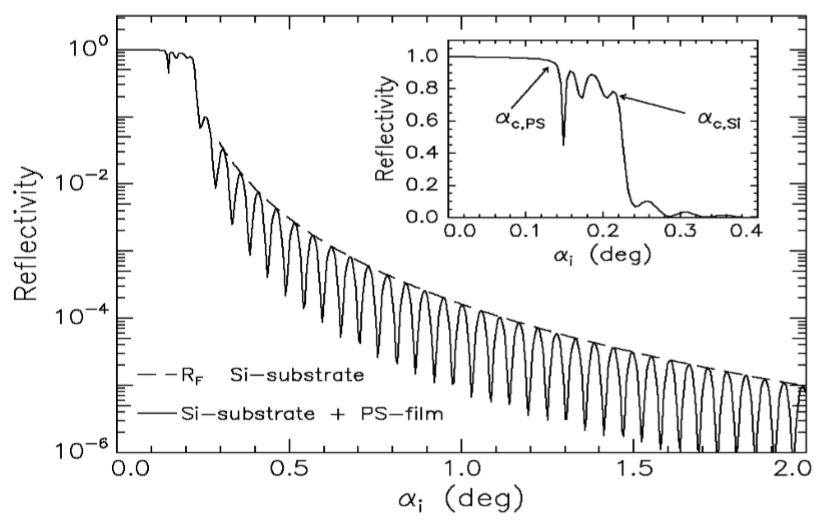
\includegraphics[width=\textwidth]{bilder/mehrschicht.png}
  \caption{Röntgenreflektivität $R$ gegen den Einfallswinkel der Strahlung $\alpha_i$ aufgetragen für ein Beispiel einer Polystyrolschicht auf einem Siliziumwafer\cite{anleitung}.}
  \label{mehrschicht}
\end{figure}
Wenn ein Mehrschichtsystem untersucht wird, müssen die jeweiligen Effekte an jeder einzelnen Grenzschicht berücksichtigt werden. Somit kommt es zu Mehrfachreflexionen mit einem reflektierten und einem transmittierten Anteil. Um dies auswerten zu können, bedient man sich des Parratt-Algorithmus. Dieser ist ein iteratives Vorgehen, um ein Mehrschichtsystem zu beschreiben und numerisch auswerten zu können.
Eine Darstellung eines solchen Mehrschichtsystems ist in Abb.\ref{parratt} zu sehen.
Als Startpunkt der Iteration wird die unterste Schicht gewählt, wo die transmittierte Schicht an keiner weiteren Schicht reflektiert wird und somit Null ist. Von der untersten bis zu obersten Schicht lassen sich nun die Verhältnisse der Amplituden zwischen transmittierter und reflektierter Strahlung über
\begin{equation}
X_j=\frac{R_j}{T_j}=e^{-2ik_{z,j}z_j}\frac{r_{j,j+1}+X_{j+1}e^{2ik{z,j+1}z_j}}{1+r_{j,j+1}+X_{j+1}e^{2ik{z,j+1}z_j}}
\end{equation}
berechnen.\\
$r_{j,j+1}=\frac{k_{z,j}-k_{z,j+1}}{k_{z,j}+k_{z,j+1}}$ ist hierbei die Fresnelreflektivität der $j$-ten Grenzfläche mit der z-Komponente des Wellenvektors $K_{z,j}=k\bigl(n_j^2-\cos^2(\alpha_i)\bigr)^{\frac{1}{2}}$ der $j$-ten Schicht.
\subsection{Rauigkeit}
Berücksichtigt werden muss bei einem experimentellen Vorgehen, dass in den bisherigen Betrachtungen von ideal glatten Ober- und Grenzflächen ausgegangen wurde. Um diese Unsicherheit für eine reale Messung zu berücksichtigen, werden angepasste Fresnelkoeffizienten
\begin{align}
  \tilde{r}_{j,j+1}&=r_{j,j+1}e^{-2k_{z,j}k_{z,j+1}\sigma_j^2}\\
  \tilde{t}_{j,j+1}&=t_{j,j+1}\exp\biggl(\frac{(k_{z,j}-k_{z,j+1}^2\sigma_j^2)}{2}\biggr)
\end{align}
verwendet. Durch diese an reale Bedingungen angepassten Fresnelkoeffizienten kann nun mit dem Parratt-Algorithmus gearbeitet werden.
\begin{figure}[H]
  \centering
  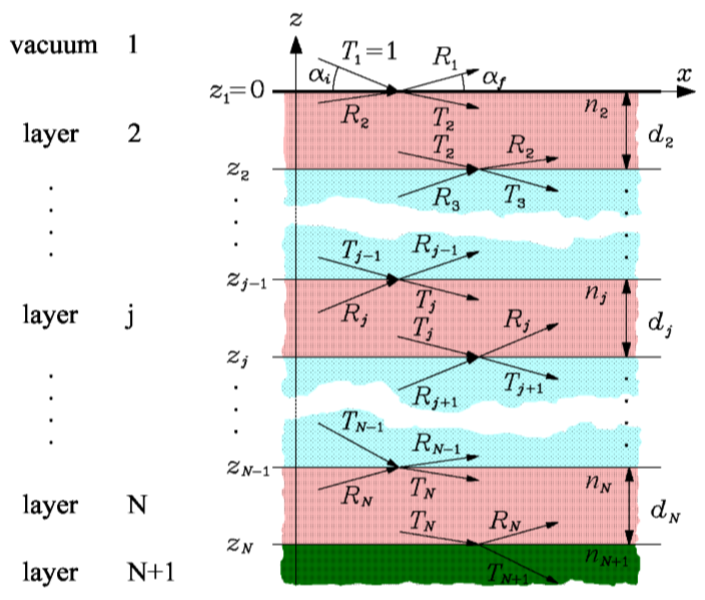
\includegraphics[width=0.7\textwidth]{bilder/parratt.png}
  \caption{Mehrschichtsystem für $N$ Grenzschichten zwischen $N+1$ Schichten mit unterschiedlichen Brechungsindizes\cite{anleitung}.}
  \label{parratt}
\end{figure}
